\documentclass[13pt]{beamer}
\usetheme{Frankfurt}
\usecolortheme{beaver}

\usepackage[spanish]{babel}
\usepackage{amsmath}
\usepackage{amsfonts}
\usepackage{amssymb}
\usepackage{color}
\usepackage{xcolor}
\usepackage{listings}
\usepackage{graphicx}
\usepackage{wrapfig}
\usepackage{algorithm2e}

\definecolor{codegreen}{rgb}{0,0.6,0}
\definecolor{codegray}{rgb}{0.5,0.5,0.5}
\definecolor{codepurple}{rgb}{0.58,0,0.82}
\definecolor{backcolour}{rgb}{0.95,0.95,0.92}

\lstdefinestyle{mystyle}{
    basicstyle=\tiny,
    commentstyle=\color{codegreen},
    keywordstyle=\color{magenta},
    numberstyle=\tiny\color{codegray},
    stringstyle=\color{codepurple},
    basicstyle=\ttfamily\footnotesize,
    breakatwhitespace=false,         
    breaklines=true,                 
    captionpos=b,                    
    keepspaces=true,                 
    numbers=left,                    
    numbersep=5pt,                  
    showspaces=false,                
    showstringspaces=false,
    showtabs=false,                  
    tabsize=2,
	xleftmargin=8pt
}

\lstset{literate=
	{á}{{\'a}}1 {é}{{\'e}}1 {í}{{\'i}}1 {ó}{{\'o}}1 {ú}{{\'u}}1
	{Á}{{\'A}}1 {É}{{\'E}}1 {Í}{{\'I}}1 {Ó}{{\'O}}1 {Ú}{{\'U}}1
	{à}{{\`a}}1 {è}{{\`e}}1 {ì}{{\`i}}1 {ò}{{\`o}}1 {ù}{{\`u}}1
	{À}{{\`A}}1 {È}{{\'E}}1 {Ì}{{\`I}}1 {Ò}{{\`O}}1 {Ù}{{\`U}}1
	{ä}{{\"a}}1 {ë}{{\"e}}1 {ï}{{\"i}}1 {ö}{{\"o}}1 {ü}{{\"u}}1
	{Ä}{{\"A}}1 {Ë}{{\"E}}1 {Ï}{{\"I}}1 {Ö}{{\"O}}1 {Ü}{{\"U}}1
	{â}{{\^a}}1 {ê}{{\^e}}1 {î}{{\^i}}1 {ô}{{\^o}}1 {û}{{\^u}}1
	{Â}{{\^A}}1 {Ê}{{\^E}}1 {Î}{{\^I}}1 {Ô}{{\^O}}1 {Û}{{\^U}}1
	{ã}{{\~a}}1 {ẽ}{{\~e}}1 {ĩ}{{\~i}}1 {õ}{{\~o}}1 {ũ}{{\~u}}1
	{Ã}{{\~A}}1 {Ẽ}{{\~E}}1 {Ĩ}{{\~I}}1 {Õ}{{\~O}}1 {Ũ}{{\~U}}1
	{œ}{{\oe}}1 {Œ}{{\OE}}1 {æ}{{\ae}}1 {Æ}{{\AE}}1 {ß}{{\ss}}1
	{ű}{{\H{u}}}1 {Ű}{{\H{U}}}1 {ő}{{\H{o}}}1 {Ő}{{\H{O}}}1
	{ç}{{\c c}}1 {Ç}{{\c C}}1 {ø}{{\o}}1 {å}{{\r a}}1 {Å}{{\r A}}1
	{€}{{\euro}}1 {£}{{\pounds}}1 {«}{{\guillemotleft}}1
	{»}{{\guillemotright}}1 {ñ}{{\~n}}1 {Ñ}{{\~N}}1 {¿}{{?`}}1 {¡}{{!`}}1 
}

\lstset{style=mystyle, basicstyle=\scriptsize}

\author{Shao Jie Hu Chen \and Mario Megías Mateo \and Jesús Samuel García Carballo}
\title{Práctica 3. Algoritmos Voraces}
\subtitle{Algorítmica}
%\logo{
\includegraphics[scale=0.05]{logo-ugr.jpeg}}
\institute{Equipo Rojo}
%\date{}
%\subject{}
%\setbeamercovered{transparent}
\setbeamertemplate{navigation symbols}{}

\begin{document}
	
	\begin{frame}[plain]
		\maketitle
		% \begin{center}
		% 	
\includegraphics[scale=0.15]{logo-ugr.jpeg}
		% \end{center}
	\end{frame}
	
	\begin{frame}
		\frametitle{Índice de contenidos}
		\tableofcontents
	\end{frame}

    % Introducción

    \section{Introducción}

    \begin{frame}
		\frametitle{Ejercicio-1}
		En este ejercicio dado un buque mercante cuya capacidad de carga es de K toneladas y un conjunto de contenedores $c_1,...,c_n$ cuyos
		pesos respectivos son $p_1,...,p_n$, debemos hallar un algoritmo que maximice el número de contenedores cargados y otro que intente 
		maximizar el número de toneladas cargadas.
	\end{frame}

    \begin{frame}
		\frametitle{Máximo número de contenedores}
		\begin{center}
			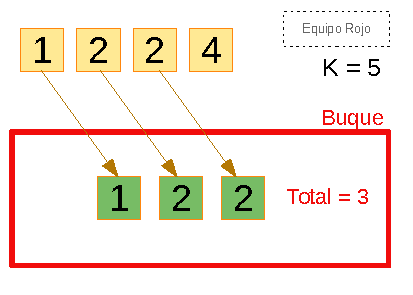
\includegraphics[scale=1.5]{./img/DibCont1.pdf}
		\end{center}
	\end{frame}

	\begin{frame}
		\frametitle{Pseudocódigo}
		\begin{algorithm}[H]
			\begin{minipage}{0.92\textwidth}
			\textbf{Parámetro}: contenedores (vector de enteros)
		
			\textbf{Parámetro}: K (capacidad del buque)
		
			\end{minipage}
		
			peso = 0\;
			vector resultado\;
			lleno = false\;
		
			sort(pesos.begin(), pesos.end());

			\For{i desde 0 hasta contenedores.tamaño-1 y !lleno} {
				\eIf{contenedores$[i]$ + peso $\leq$ K}{
					peso += contenedores$[i]$\;
				}{ lleno = true\;}
			}

			\Return{result}
			
		\end{algorithm}
	\end{frame}

    \begin{frame}
		\frametitle{Máximas toneladas}
		\begin{center}
			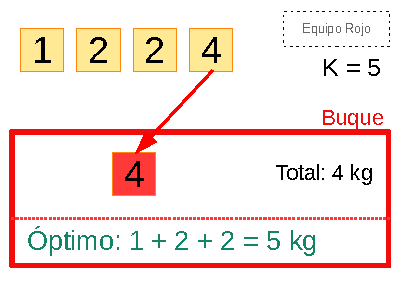
\includegraphics[scale=1.5]{./img/DibCont2.pdf}
		\end{center}
	\end{frame}

	\begin{frame}
		\frametitle{Pseudocódigo}
		\begin{algorithm}[H]
			\caption{Algoritmo para maximizar las toneladas}\label{alg:max_toneladas}
			\begin{minipage}{0.92\textwidth}
		
			\textbf{Parámetro}: containers (vector de enteros)
		
			\textbf{Parámetro}: K (capacidad del buque)
		
			\end{minipage}
		
			weight = 0\;
			container = 0\;
			vector result\;
		  
			sort(containers.begin(),containers.end(),greater$<$int$>$());
		
			\While{$weight  \leq K$ y $container  \leq containers.size$}{      
				\If{$weight + containers.at(container) \leq K$}{
					result.push\_back(containers.at(container))\;
					$weight += containers.at(container)$\;
				}
				container++\;
			}
		  
		
			\Return{result}
		\end{algorithm}
	\end{frame}

    \begin{frame}
		\frametitle{Problema del Viajante del Comercio}

        \begin{itemize}
            \item Algoritmo del vecino más cercano.
            \item Algoritmo de inserción económica.
            \item Algoritmo basado en Kruskal.
        \end{itemize}

	\end{frame}

    \begin{frame}
		\frametitle{Algoritmo del vecino más cercano}
		\begin{center}
			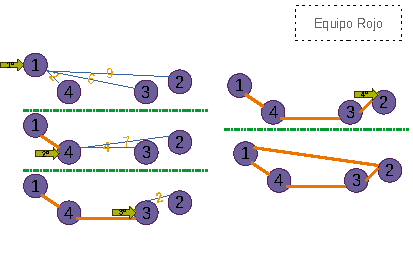
\includegraphics[scale=1.5]{./img/DibVecCercano.pdf}
		\end{center}
	\end{frame}

	\begin{frame}
		\frametitle{Pseudocódigo}

	\end{frame}

	\begin{frame}
		\frametitle{Algoritmo del vecino más cercano}
			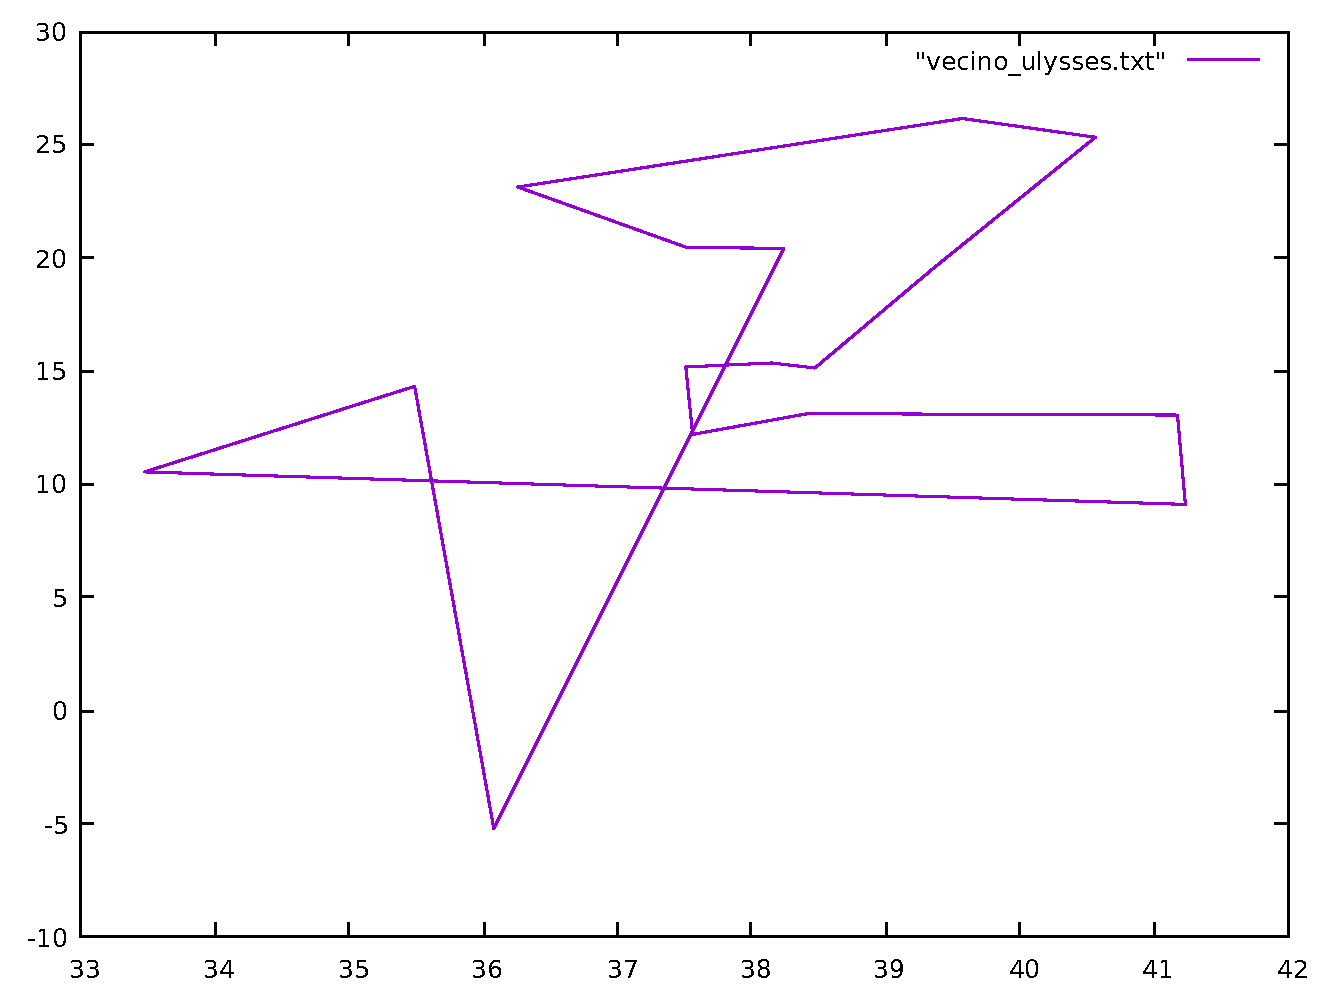
\includegraphics[scale=0.2]{../src/vecino_ulysses.pdf}
			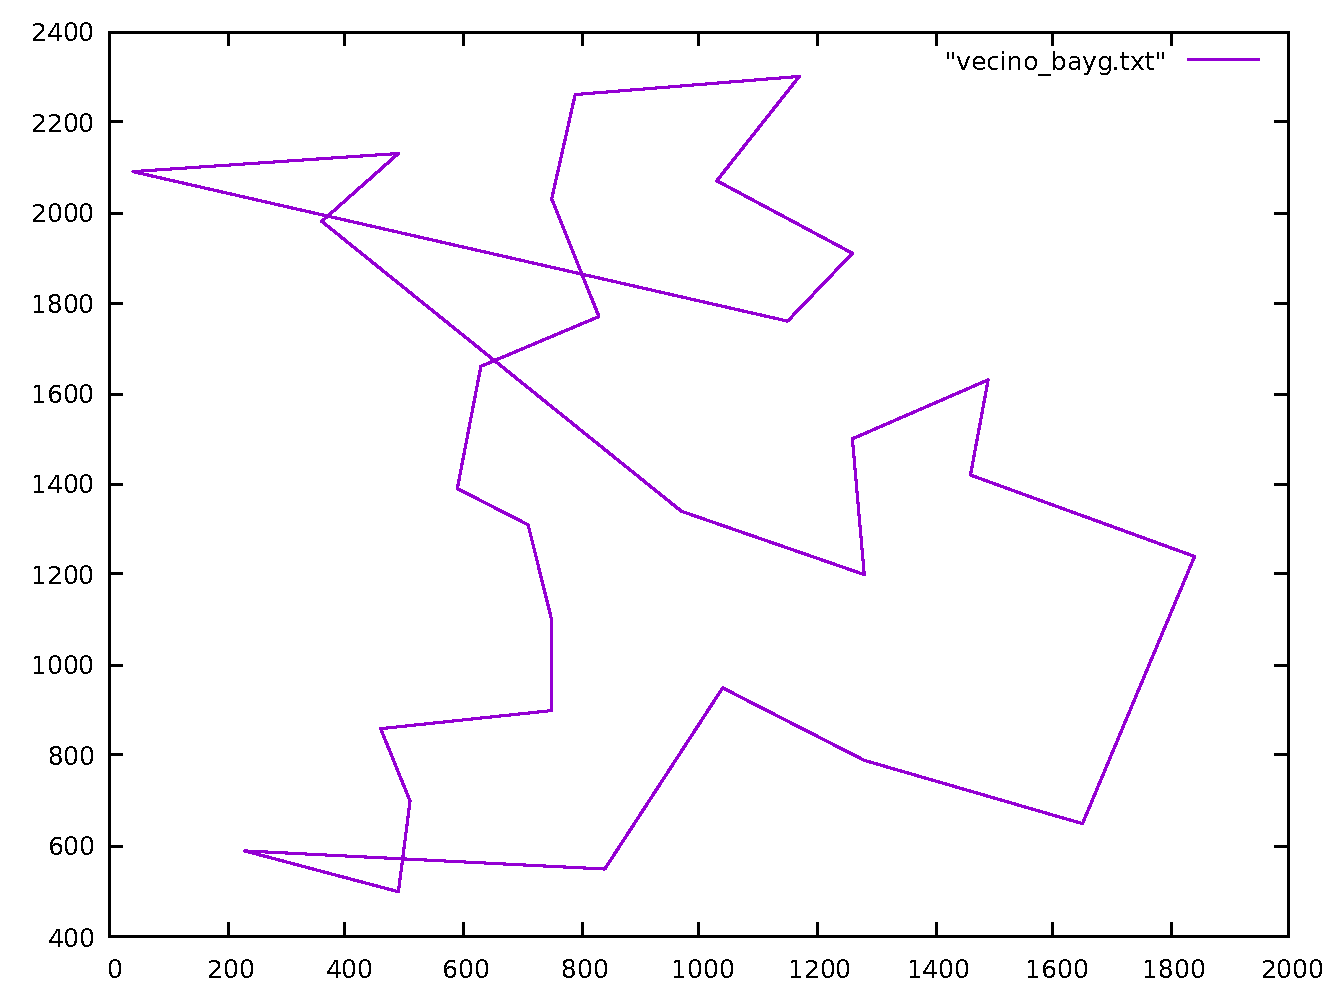
\includegraphics[scale=0.2]{../src/vecino_bayg.pdf}
			\begin{center}
				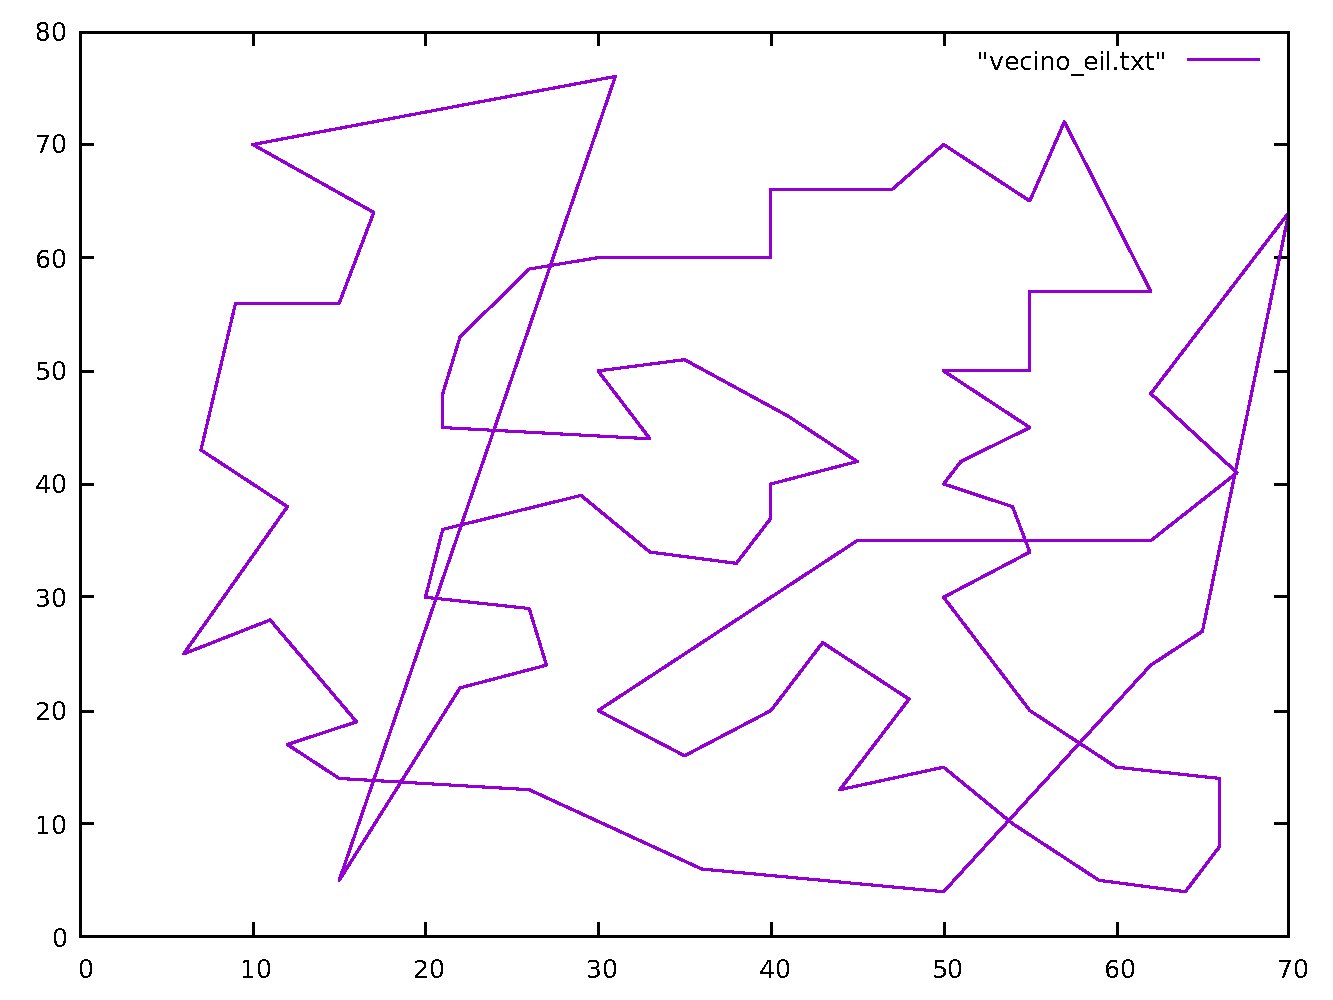
\includegraphics[scale=0.2]{../src/vecino_eil.pdf}
			\end{center}
	\end{frame}


    \begin{frame}
		\frametitle{Algoritmo de inserción económica}
		\begin{center}
			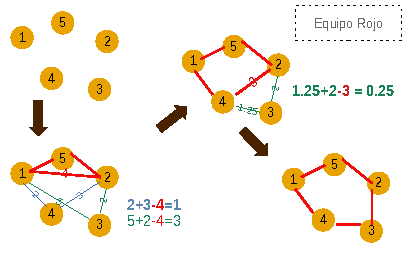
\includegraphics[scale=1.5]{./img/DibInsercion.pdf}
		\end{center}
	\end{frame}

	\begin{frame}
		\frametitle{Pseudocódigo}
		
	\end{frame}

	\begin{frame}
		\frametitle{Algoritmo del vecino más cercano}
			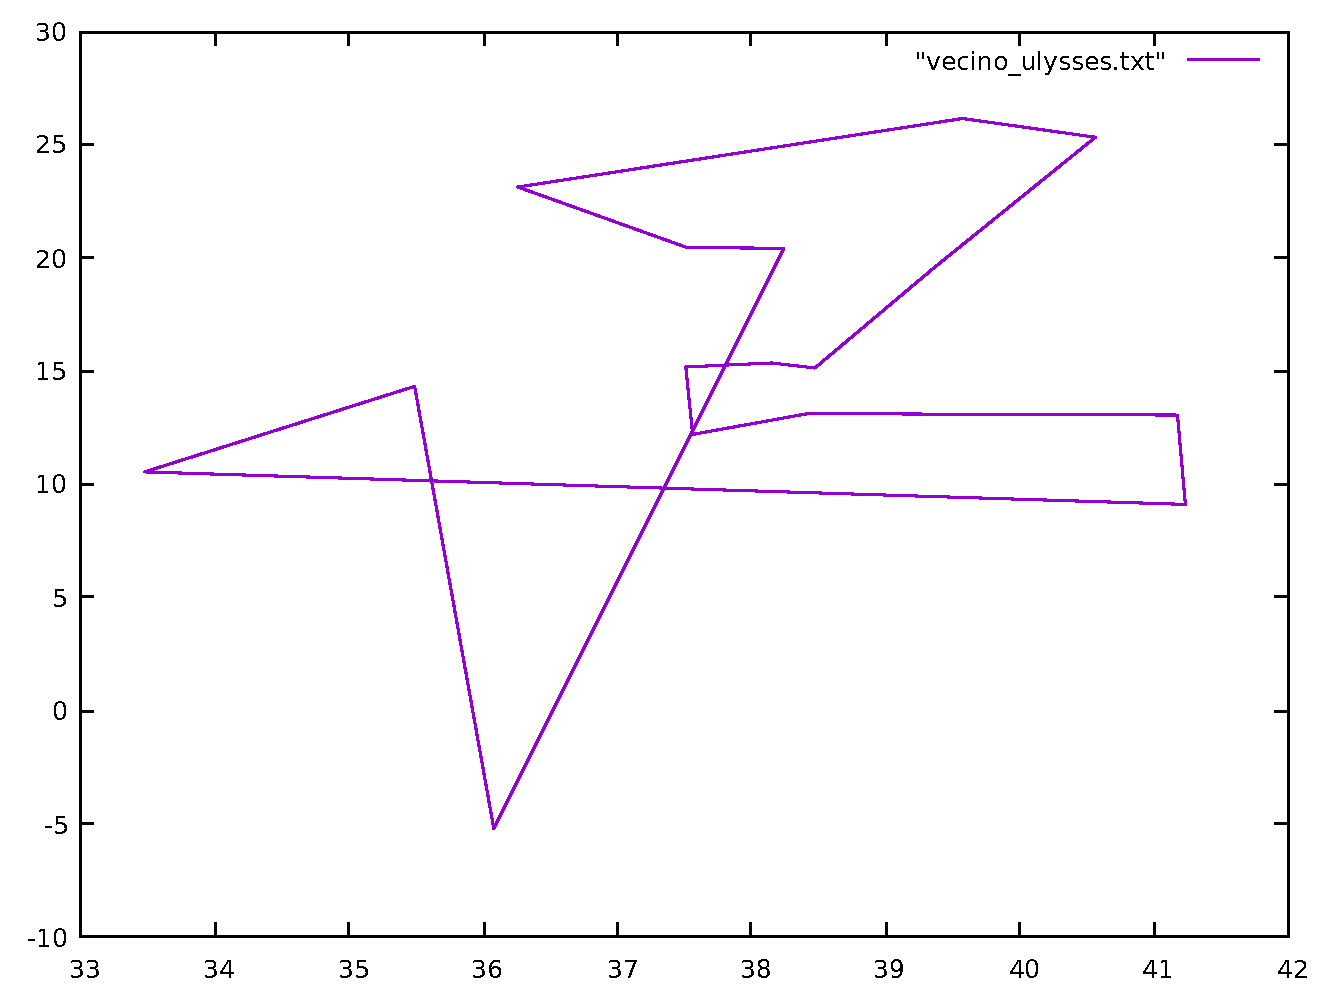
\includegraphics[scale=0.2]{../src/vecino_ulysses.pdf}
			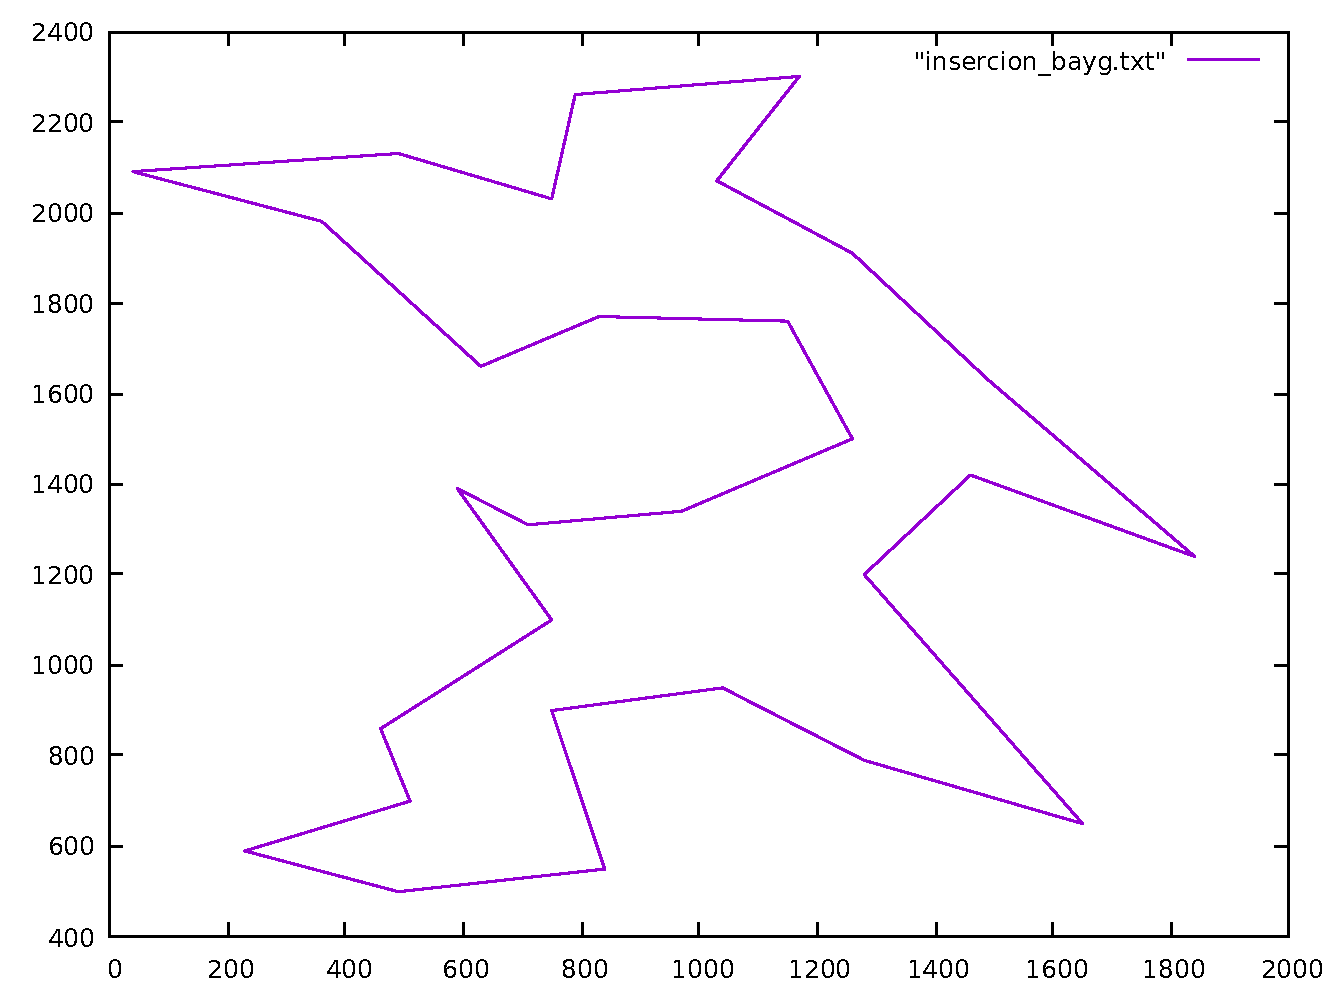
\includegraphics[scale=0.2]{../src/insercion_bayg.pdf}
			\begin{center}
				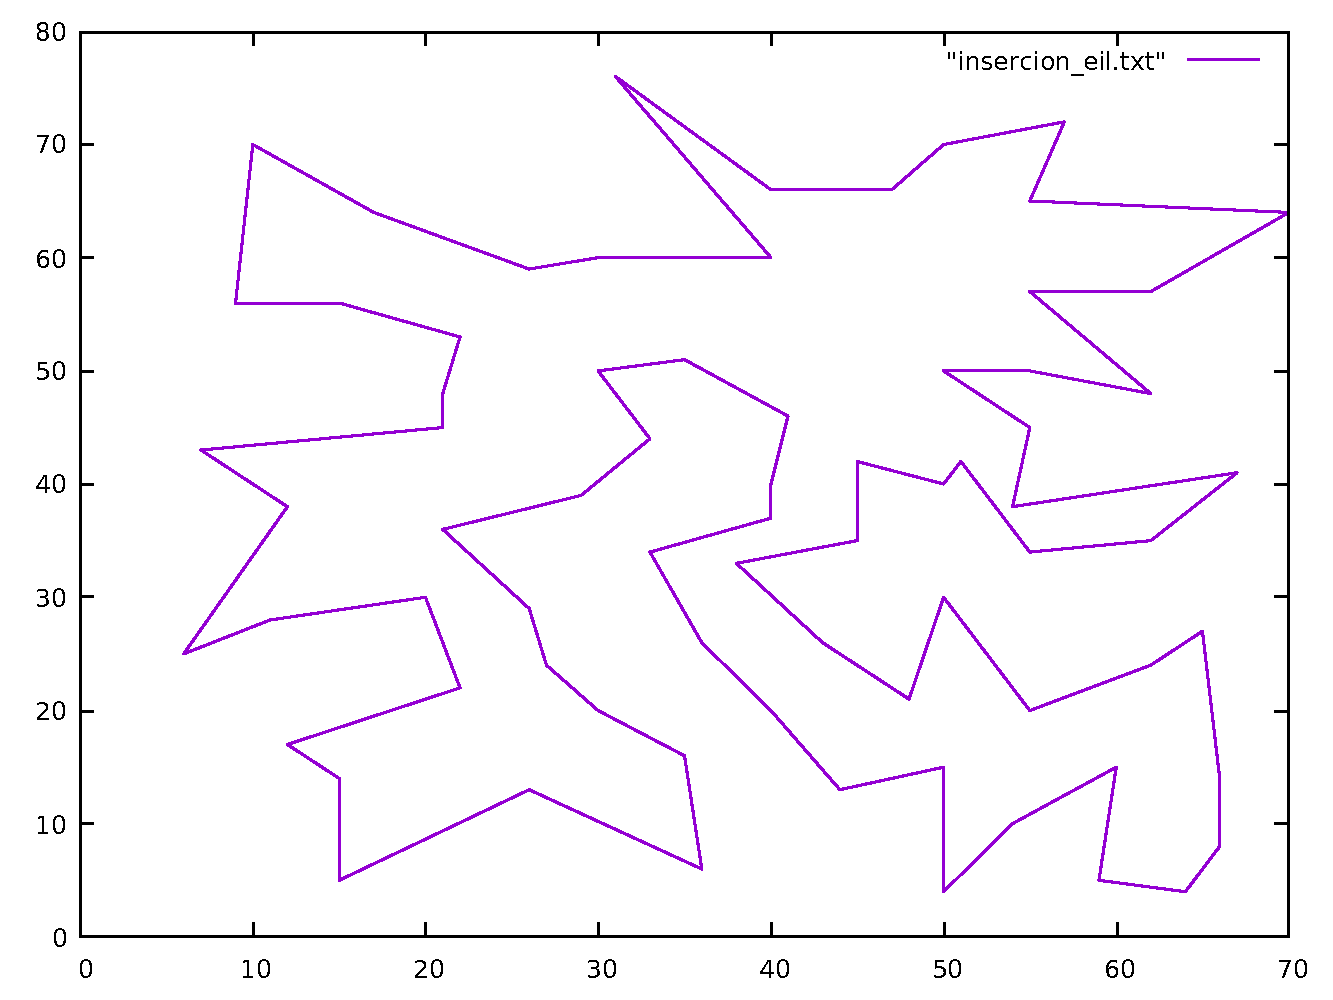
\includegraphics[scale=0.2]{../src/insercion_eil.pdf}
			\end{center}
	\end{frame}

    \begin{frame}
		\frametitle{Algoritmo basado en Kruskal}
		\begin{center}
			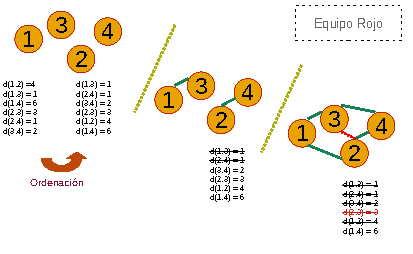
\includegraphics[scale=1.5]{./img/DibPropio.pdf}
		\end{center}
	\end{frame}

	\begin{frame}
		\frametitle{Pseudocódigo}

	\end{frame}

	\begin{frame}
		\frametitle{Algoritmo del vecino más cercano}
			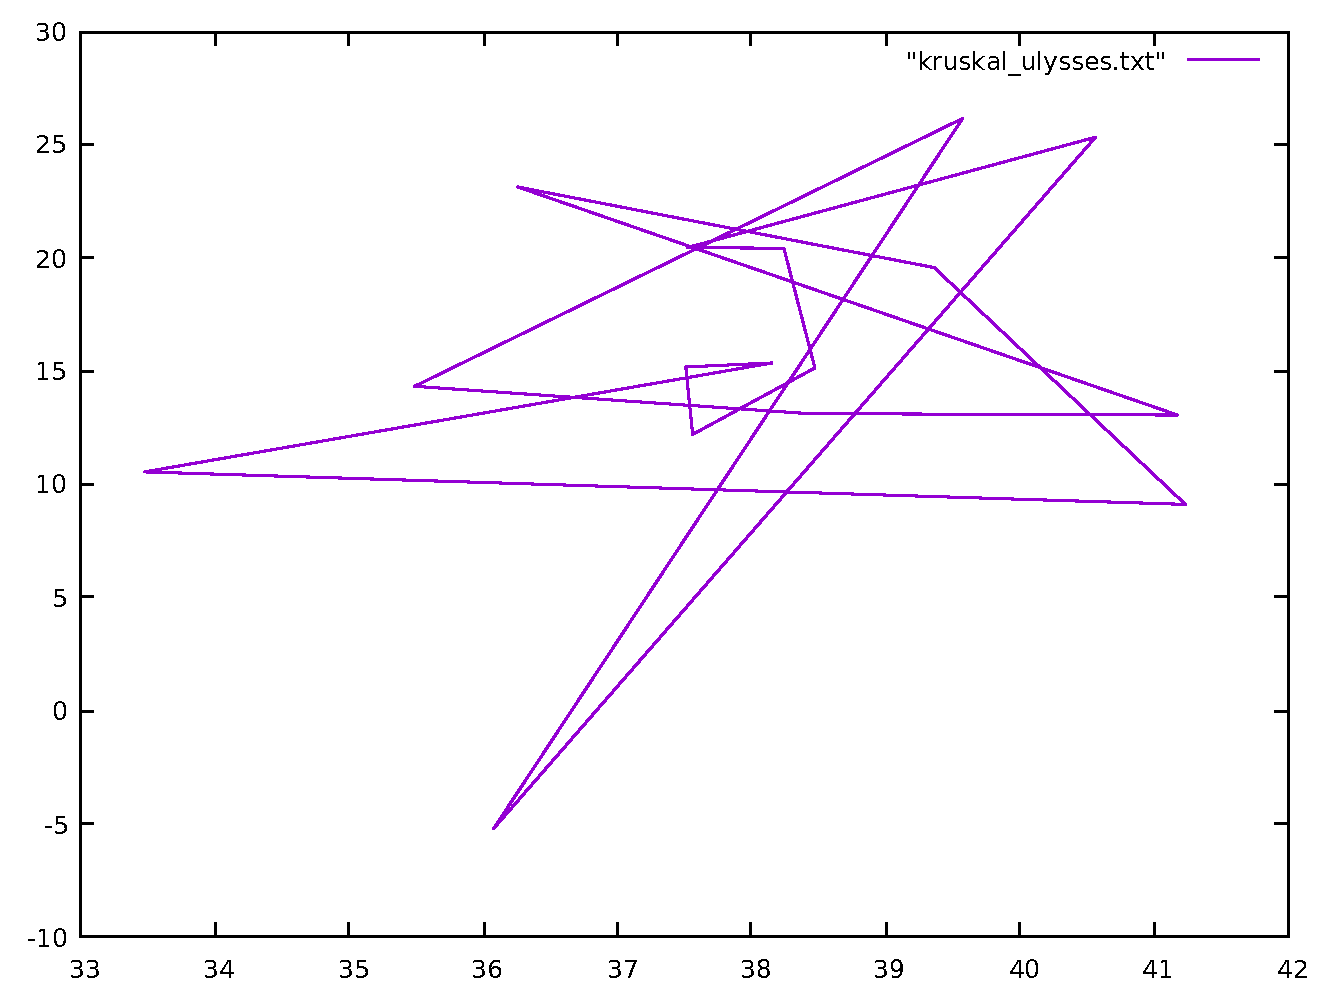
\includegraphics[scale=0.2]{../src/kruskal_ulysses.pdf}
			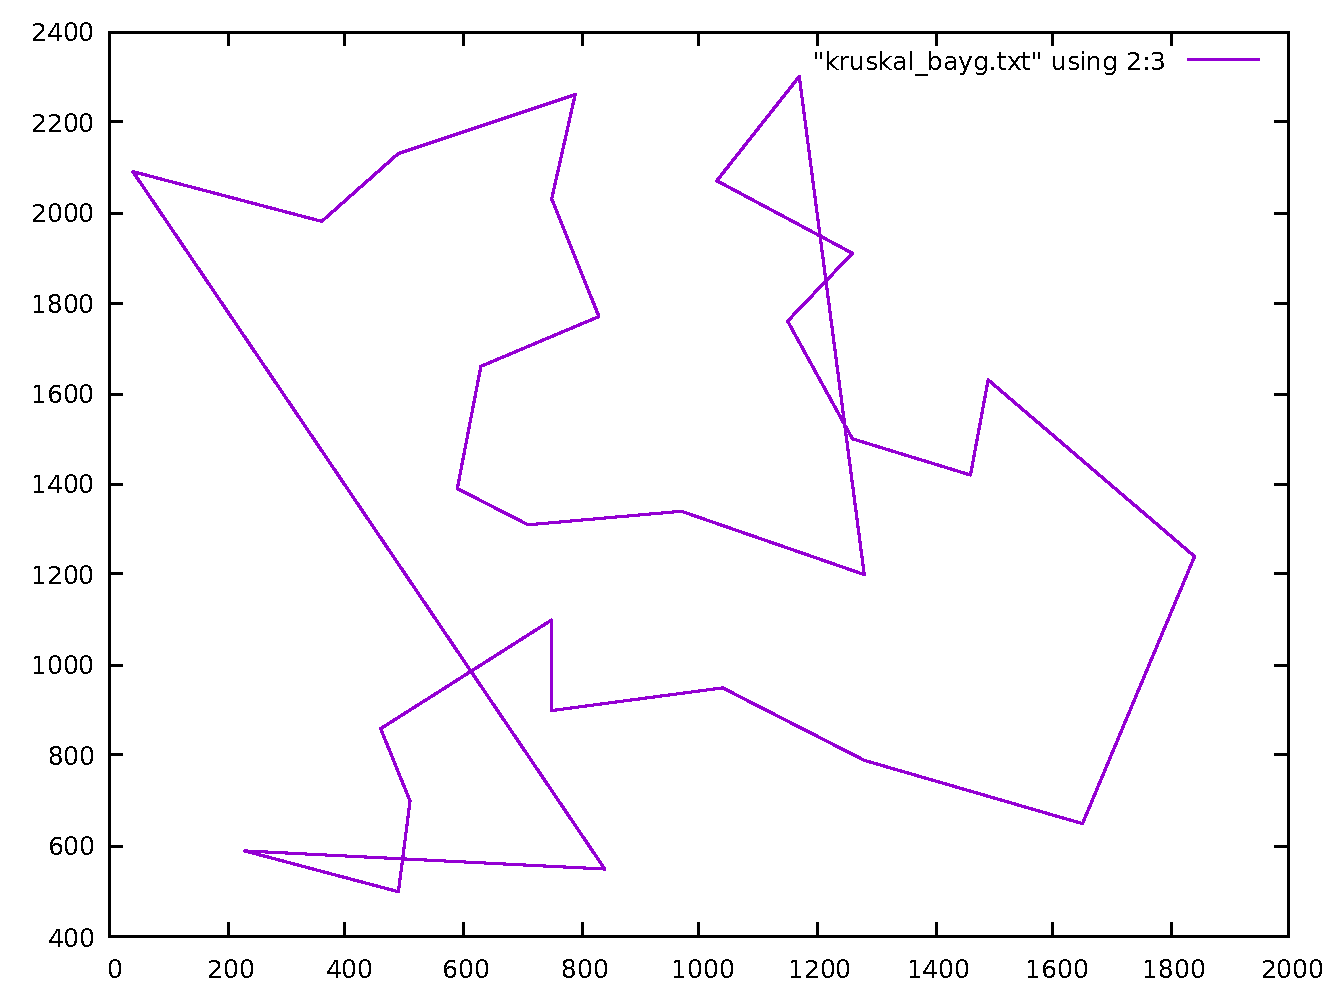
\includegraphics[scale=0.2]{../src/kruskal_bayg.pdf}
			\begin{center}
				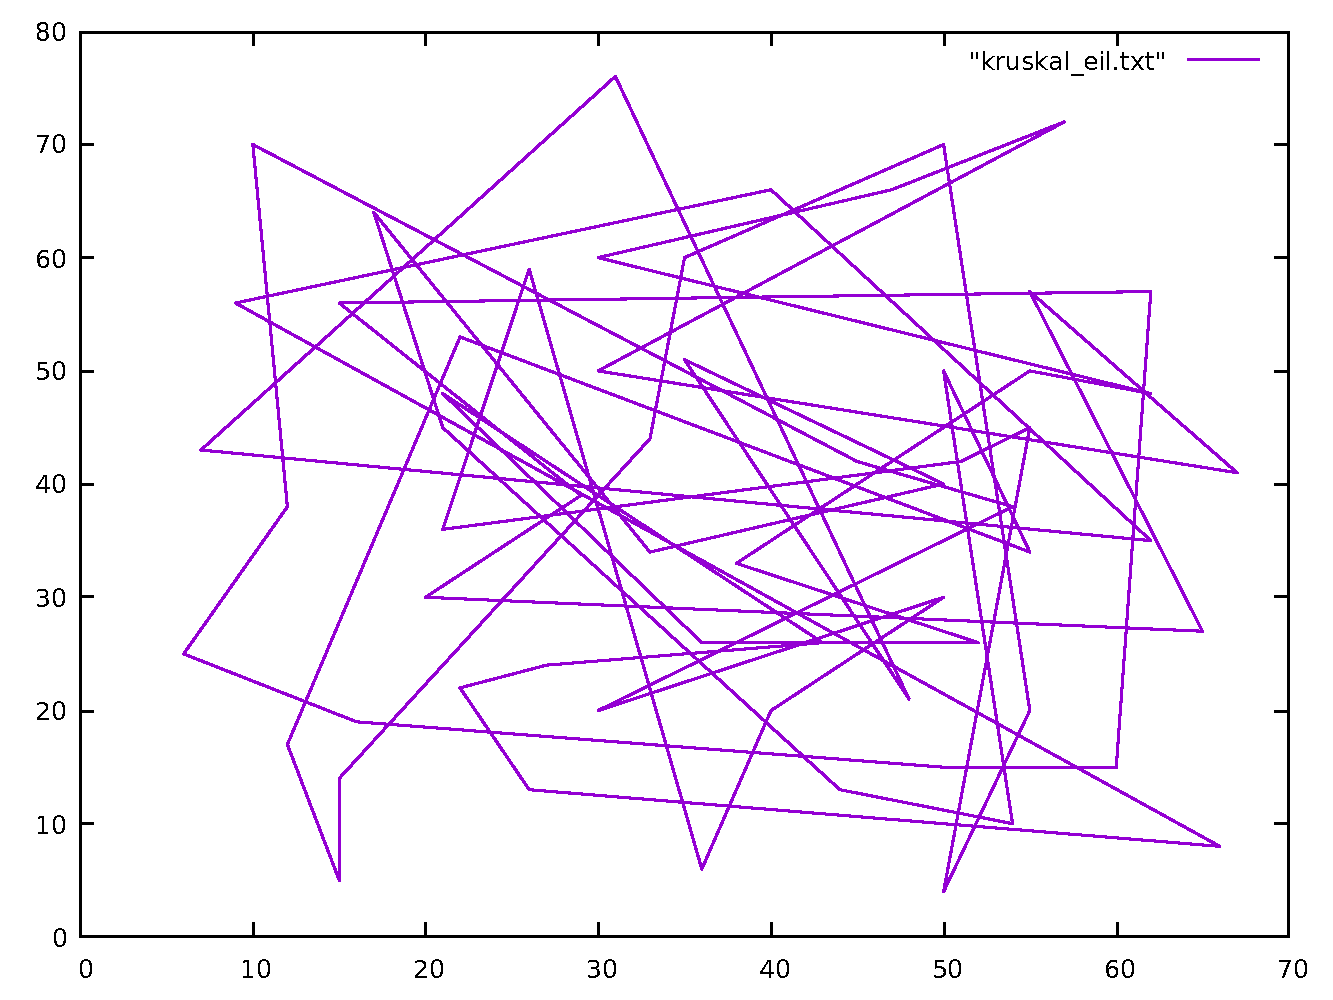
\includegraphics[scale=0.2]{../src/kruskal_eil.pdf}
			\end{center}
	\end{frame}

    \begin{frame}
		\frametitle{Conclusion}
			\begin{itemize}
				\item Conocer y trabajar con algoritmos greedy, comprendiendo su enfoque.
				\item Comprender el problema del TSP, uno de los más importantes en materia de algorítmica y saber trabajar con el, para proporcionar soluciones.
				\item Estudiar la eficiencia de distintos algoritmos del problema del Viajante de Comercio.
				\item Entender y saber utilizar grafos, así como la matriz de adyacencia, ambos aplicados a la resolución de problemas.
			\end{itemize}		
	\end{frame}

    % Bibliografía

    \section{Bibliografía}

    \begin{frame}
        \begin{thebibliography}{0}
            \bibitem{Verdegay2017} Verdegay Galdeano. (2017). Lecciones de Algorítmica / José Luis Verdegay. Técnica Avicam.
            \bibitem{Cormen2017} Cormen. (2017). Introduction to algorithms / Thomas H. Cormen... [et al.] (3rd ed.). PHI Learning.
            \bibitem{Garrido2018} Garrido Carrillo. (2018). Estructuras de datos avanzadas: con soluciones en C++ / A. Garrido. Universidad de Granada.  
        \end{thebibliography}
    \end{frame}

\end{document}